\chapter{The Question: Can a Fitted Potential Learn the Riemann Zeros?}\label{ch:intro}

\begin{chapterintro}
Here is a list of numbers: $14.134725$, $21.022040$, $25.010858$, $30.424876$, $32.935062$, and it goes on forever. Mathematicians have studied these numbers for more than a century and a half. They are built, in a way we will make precise later in the book, out of the prime numbers. Physicists have stared at the same list and seen something familiar: the numbers are spread out the way the allowed energies of a quantum system are spread out. That observation has fed a hope, still unproved, that somewhere there is a quantum system whose energy levels are exactly these numbers.

One way to chase that hope is purely empirical. You take a quantum particle trapped in a valley of potential energy, and you adjust the shape of the valley until its allowed energies match the list. If you can make them match very well, have you found something? Or have you only bent a flexible curve until it passed through your data points? This book is about how to tell the difference, and about one research paper \cite{soniR1} that asked exactly this question and answered it with a held-out test.

In this chapter we meet the numbers, see roughly where they come from, see why they look like energy levels, and learn in plain language what it means to fit a model, to memorize, and to predict. We finish with the paper's result in one page and a road map of the book. Where this shows up in the paper: the abstract, Fig.~1, and all of Sec.~I (the Introduction and its four strands of prior work, Sec.~I~A).
\end{chapterintro}

\begin{prerequisites}
\item First-year physics: potential energy curves and turning points (a ball rolling in a valley turns around where its kinetic energy reaches zero).
\item First-year physics: standing waves on a string with fixed ends and their harmonics.
\item Calculus basics: logarithms (always the natural logarithm $\log$ in this book), exponentials, and the value $\pi = 3.14159\ldots$
\item Arithmetic averages (the mean of a list of numbers) and squares and square roots.
\item No earlier chapter is assumed. Everything else is introduced here in words and developed properly later.
\end{prerequisites}

%======================================================================
\section{A list of mysterious numbers}\label{sec:intro-numbers}

Let us start with the data, the way an experimentalist would. \Cref{tab:intro-first10} lists the first ten numbers of our list. We call the $n$-th number $t_n$, so $t_1 = 14.134725$, $t_2 = 21.022040$, and so on. The index $n$ is a counting label: $n = 1, 2, 3, \ldots$. These ten values are the first running example of the book (RE1), and you will see them again and again.

\begin{table}[htbp]\centering
\caption{The first ten heights $t_n$ of the nontrivial Riemann zeros (running example RE1), rounded to six decimal places, and the spacing $t_{n+1}-t_n$ to the next one.}
\label{tab:intro-first10}
\begin{tabular}{ccc}
\toprule
$n$ & $t_n$ & $t_{n+1}-t_n$ \\
\midrule
1 & 14.134725 & 6.887315 \\
2 & 21.022040 & 3.988818 \\
3 & 25.010858 & 5.414018 \\
4 & 30.424876 & 2.510186 \\
5 & 32.935062 & 4.651116 \\
6 & 37.586178 & 3.332541 \\
7 & 40.918719 & 2.408354 \\
8 & 43.327073 & 4.678078 \\
9 & 48.005151 & 1.768681 \\
10 & 49.773832 & \\
\bottomrule
\end{tabular}
\end{table}

What do you notice? The numbers increase. They are not equally spaced: the gaps jump around between about $1.8$ and $6.9$. There is no obvious formula like ``add 4 each time''. And yet they are not completely haphazard either: among these ten no gap is extremely small (small gaps are observed numerically to be rare at all heights computed, \cref{sec:intro-hp}), and on average the numbers come a little closer together as you go up. The paper you will learn to read uses the first $10^4$ of them for its explicit-formula oracle and its spacing statistics (paper Table~V, Fig.~2) and at most the first 1000 in its fitted potentials; its zero number 1000 is $t_{1000} = 1419.42248\ldots$ (paper Sec.~II~A).

These numbers are called the \emph{heights of the nontrivial zeros of the Riemann zeta function}. We will explain each word of that phrase in \cref{sec:intro-primes}. For now, treat them as measured data: a long, precise list that someone has handed you.

\begin{sample}{Reading the spacings of the first ten zeros}
Using \cref{tab:intro-first10}, find the average spacing between consecutive zeros among the first ten, and the largest and smallest spacings.

\textbf{Step 1:} There are ten zeros, so there are nine spacings between consecutive ones: $t_2-t_1$, $t_3-t_2$, up to $t_{10}-t_9$.

\textbf{Step 2:} The sum of the nine spacings telescopes: every intermediate $t_n$ appears once with a plus sign and once with a minus sign, so
\[
(t_2 - t_1) + (t_3 - t_2) + \cdots + (t_{10}-t_9) = t_{10} - t_1 = 49.773832 - 14.134725 = 35.639107 .
\]

\textbf{Step 3:} The average spacing is the sum divided by the number of spacings:
\[
\frac{35.639107}{9} = 3.959901 .
\]

\textbf{Step 4:} Reading down the last column of the table, the largest spacing is $t_2 - t_1 = 6.887315$ and the smallest is $t_{10}-t_9 = 1.768681$.

\textbf{Answer:}
\[
\boxed{\text{average spacing} = 3.959901,\quad \text{largest} = 6.887315,\quad \text{smallest} = 1.768681}
\]
\end{sample}

\subsection{Counting the zeros: a staircase}

A second way to look at a list of increasing numbers is to count. Define $N(T)$, read ``N of T'', as the number of zeros whose height $t$ satisfies $0 < t \le T$:
\begin{equation}
N(T) = \text{(number of } n \text{ with } t_n \le T\text{)} .
\label{eq:intro-NT}
\end{equation}
Below $T = 14.134725$ there are no zeros, so $N(T) = 0$ there. At $T = t_1$ the count jumps to 1 and stays at 1 until $T = t_2$, where it jumps to 2, and so on. Plotted against $T$, $N(T)$ is a staircase with a step of height 1 at each zero (\cref{fig:intro-staircase}).

Here is a remarkable fact, which we take on trust now and derive in Chapter~\ref{ch:counting-zeros}. The staircase hugs a smooth curve,
\begin{equation}
\Nsm(t) = \frac{t}{2\pi}\log\frac{t}{2\pi} - \frac{t}{2\pi} + \frac78 ,
\label{eq:intro-Nsm}
\end{equation}
which is Eq.~(1) of the paper. The subscript ``sm'' stands for ``smooth''. The staircase wobbles around this curve, sometimes a little above it, sometimes a little below, but it never wanders far. The wobble is the interesting part. It is where the primes hide.

\begin{figure}[htbp]\centering
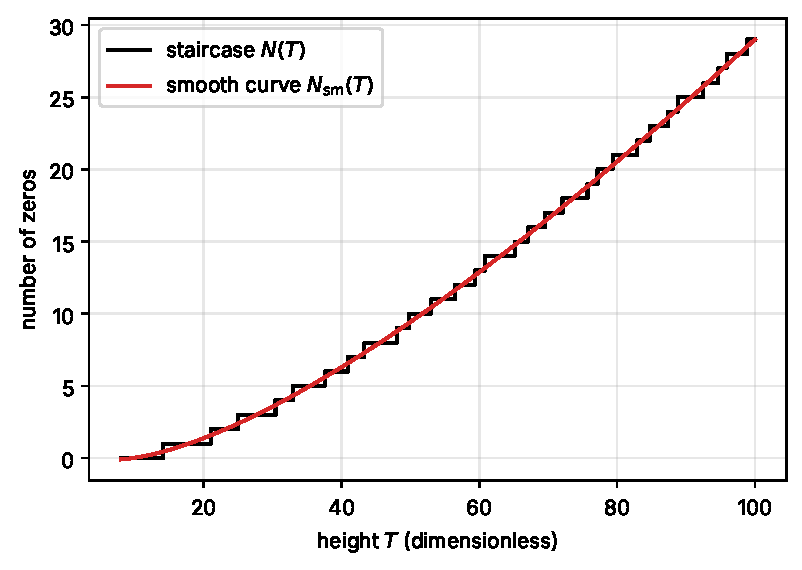
\includegraphics[width=0.85\linewidth]{figs/intro_staircase.pdf}
\caption{The counting staircase $N(T)$ of \cref{eq:intro-NT}, which steps up by 1 at each zero height $t_n$, and the smooth curve $\Nsm(T)$ of \cref{eq:intro-Nsm} (paper Eq.~(1)) for $8 \le T \le 100$. The staircase oscillates around the smooth curve; in this range the departure stays below one step (checked numerically in this chapter's code).}
\label{fig:intro-staircase}
\end{figure}

\begin{sample}{The staircase against the smooth curve}
Find $N(50)$ and $N(100)$, and compare with $\Nsm(50)$ and $\Nsm(100)$. You are told that the eleventh zero is $t_{11} = 52.970321$, the twenty-ninth is $t_{29} = 98.831194$ and the thirtieth is $t_{30} = 101.317851$.

\textbf{Step 1: count.} From \cref{tab:intro-first10}, $t_{10} = 49.773832 \le 50$ and $t_{11} = 52.970321 > 50$, so exactly ten zeros lie at or below 50: $N(50)=10$. Similarly $t_{29} \le 100 < t_{30}$ gives $N(100) = 29$.

\textbf{Step 2: the ratio $t/2\pi$.} For $t = 50$, $t/2\pi = 50/6.2831853 = 7.957747$. For $t=100$, $t/2\pi = 15.915494$.

\textbf{Step 3: the logarithms.} $\log 7.957747 = 2.074146$ and $\log 15.915494 = 2.767293$.

\textbf{Step 4: assemble \cref{eq:intro-Nsm} for $t=50$.}
\[
\Nsm(50) = 7.957747 \times 2.074146 - 7.957747 + 0.875 = 16.505528 - 7.957747 + 0.875 = 9.422781 .
\]

\textbf{Step 5: assemble for $t=100$.}
\[
\Nsm(100) = 15.915494 \times 2.767293 - 15.915494 + 0.875 = 44.042844 - 15.915494 + 0.875 = 29.002350 .
\]

\textbf{Answer:}
\[
\boxed{N(50)=10,\ \Nsm(50)\approx 9.423;\qquad N(100)=29,\ \Nsm(100)\approx 29.002}
\]
At $T=50$ the staircase sits about $0.58$ steps above the smooth curve; at $T=100$ it sits almost exactly on it. The difference $N(T) - \Nsm(T)$ is the wobble.
\end{sample}

\subsection{The mean spacing and the fluctuations}

Because the staircase follows $\Nsm$, the smooth curve tells you how densely the zeros are packed near any height. If the curve climbs by one unit over a stretch of length $\ell$ in $t$, then on average one zero sits in that stretch, so the average spacing there is $\ell$. The slope of the smooth curve is
\[
\Nsm'(t) = \frac{1}{2\pi}\log\frac{t}{2\pi} + \frac{t}{2\pi}\cdot\frac{1}{t} - \frac{1}{2\pi} = \frac{1}{2\pi}\log\frac{t}{2\pi}
\]
(the product rule on the first term of \cref{eq:intro-Nsm}, using $\frac{\dd}{\dd t}\log\frac{t}{2\pi} = \frac1t$, produces a $+\frac{1}{2\pi}$ that cancels the $-\frac{1}{2\pi}$ from the second term). So one unit of climb takes a stretch $\ell \approx 1/\Nsm'(t)$, provided the slope changes little over that stretch. This gives the \emph{local mean spacing}; near height $t$ it is approximately
\begin{equation}
\text{mean spacing near } t \approx \frac{2\pi}{\log(t/2\pi)} .
\label{eq:intro-gap}
\end{equation}
The paper writes this spacing as $\gap_n$ for the region near zero $n$. Since $\log(t/2\pi)$ grows as $t$ grows, the spacing shrinks slowly: the zeros crowd together as you go up, which matches what you noticed in \cref{tab:intro-first10}.

The paper also uses the \emph{smooth zeros} $s_n$: the positions where the smooth curve passes through the half-integers, $\Nsm(s_n) = n - \tfrac12$. You can think of $s_n$ as ``where zero $n$ would be if there were no wobble''. The paper defines the spacing near zero $n$ precisely as $\gap_n = \dd s_n/\dd n$, the rate at which the smooth zero moves as $n$ increases (treating $n$ as a continuous variable). Differentiating $\Nsm(s_n) = n - \tfrac12$ with respect to $n$ by the chain rule gives $\Nsm'(s_n)\,\dd s_n/\dd n = 1$, so $\gap_n = 1/\Nsm'(s_n) = 2\pi/\log(s_n/2\pi)$: exactly \cref{eq:intro-gap} evaluated at $t = s_n$ (Chapter~\ref{ch:counting-zeros} returns to this). The difference $t_n - s_n$, divided by the local mean spacing, is called the \emph{fluctuation} of zero $n$, measured in mean spacings. Typical fluctuations are a fraction of one spacing. All the predictions in the paper are predictions of these fluctuations. (For the fitted potentials the paper measures fluctuations relative to the levels of the unperturbed potential, which track $s_n$ closely; see \cref{sec:intro-memorize}.)

\begin{sample}{Measuring an error in mean spacings}
The paper reports $t_{500} = 811.1843588465$ (paper Appendix~A, key anchors). (a) Estimate the local mean spacing near zero 500 from \cref{eq:intro-gap}. (b) Express an error of $0.5$ in $t$ at that height in units of mean spacing. (c) Compare the spacing with the average spacing of the first ten zeros from the Sample Problem ``Reading the spacings of the first ten zeros''.

\textbf{Step 1:} $t/2\pi = 811.1843588/6.2831853 = 129.10399$.

\textbf{Step 2:} $\log 129.10399 = 4.860618$.

\textbf{Step 3:} Mean spacing $\approx 6.2831853/4.860618 = 1.292672$.

\textbf{Step 4:} An error of $0.5$ in $t$ is $0.5/1.292672 = 0.3868$ mean spacings.

\textbf{Step 5:} The ratio of spacings is $3.959901/1.292672 = 3.063$.

\textbf{Answer:}
\[
\boxed{\text{spacing} \approx 1.293,\quad 0.5 \text{ in } t = 0.387 \text{ spacings},\quad \text{low zeros are } 3.06\times \text{ farther apart}}
\]
The same error in $t$ is a much bigger mistake near zero 500 than near zero 5, because the zeros are packed about three times more tightly. That is why the paper quotes every error in mean spacings.
\end{sample}

\begin{sample}{Fluctuations of the first two zeros}
Find the smooth zeros $s_1$ and $s_2$, the local mean spacings there from \cref{eq:intro-gap}, and the fluctuations $(t_n - s_n)/\gap_n$ of the first two zeros.

\textbf{Step 1: rewrite the condition.} With $u = t/2\pi$, \cref{eq:intro-Nsm} reads $\Nsm = u\log u - u + \tfrac78$. The condition $\Nsm(s_1) = 1 - \tfrac12 = \tfrac12$ becomes $u\log u - u = \tfrac12 - \tfrac78 = -0.375$. Call the left side $f(u)$.

\textbf{Step 2: bracket by trial.} $f(2.30) = 2.30\times 0.832909 - 2.30 = -0.3843$, below $-0.375$; $f(2.32) = 2.32\times 0.841567 - 2.32 = -0.3676$, above it. The function $f$ increases for $u > 1$, because its derivative is $\log u + 1 - 1 = \log u > 0$ (product rule: $\frac{\dd}{\dd u}(u\log u) = \log u + 1$). Since $f$ is increasing there, it crosses $-0.375$ exactly once, and the crossing lies between $2.30$ and $2.32$.

\textbf{Step 3: refine.} $f(2.311) = 2.311\times 0.8376803 - 2.311 = -0.375121$, short of $-0.375$ by $0.000121$. Near $u = 2.311$ the slope of $f$ is $\log u = 0.838$, so $u$ must grow by a further $0.000121/0.838 = 0.000144$, giving $u = 2.311144$. (Chapter~\ref{ch:asymptotics} turns this step into Newton's method.)

\textbf{Step 4: $s_1$ and its spacing.} $s_1 = 2\pi u = 6.2831853\times 2.311144 = 14.5213$. The mean spacing is $2\pi/\log 2.311144 = 6.2831853/0.837743 = 7.500$.

\textbf{Step 5: fluctuation of zero 1.} $(14.134725 - 14.5213)/7.500 = -0.3866/7.500 = -0.0515$.

\textbf{Step 6: zero 2.} Now $f(u) = \tfrac32 - \tfrac78 = 0.625$. Trials: $f(3.28) = 3.28\times1.187843 - 3.28 = 0.6161$ (below), $f(3.29) = 3.29\times 1.190887 - 3.29 = 0.6280$ (above), $f(3.2875) = 3.2875\times 1.1901274 - 3.2875 = 0.625044$, above $0.625$ by $0.000044$. With slope $\log u = 1.190$, reduce $u$ by $0.000044/1.190 = 0.000037$, giving $u = 3.287463$, which we round to $3.28746$. Then $s_2 = 6.2831853\times 3.28746 = 20.6557$, the spacing is $6.2831853/\log 3.28746 = 6.2831853/1.19012 = 5.2795$, and the fluctuation is $(21.022040 - 20.6557)/5.2795 = 0.3663/5.2795 = 0.0694$.

\textbf{Answer:}
\[
\boxed{s_1 = 14.5213,\ \text{fluct}_1 = -0.052;\qquad s_2 = 20.6557,\ \text{fluct}_2 = +0.069}
\]
The first zero sits a little below its smooth position, the second a little above; both displacements are a small fraction of one spacing. The library call \texttt{qmnt.fluct(qmnt.zeros(2), np.array([1, 2]))} returns the same two numbers.
\end{sample}

\begin{pitfall}
Do not compare raw errors in $t$ across different heights. An error of $0.5$ is about one eighth of a spacing near $t=30$ but nearly two fifths of a spacing near $t = 811$. The paper's rms values (Tables~I--V) are all in units of the local mean spacing, so that a number like $0.263$ means the same thing at every height.
\end{pitfall}

\begin{pycode}
import numpy as np
import qmnt

t = qmnt.zeros(10)          # first ten zero heights t_1..t_10
print(t)

gaps = t[1:] - t[:-1]       # nine spacings
print("mean spacing:", gaps.mean())
print("largest, smallest:", gaps.max(), gaps.min())

T = 100.0
print("N(100) =", np.sum(qmnt.zeros(40) <= T))
print("Nsm(100) =", qmnt.Nsm(T))
\end{pycode}

\begin{checkpoint}
Two zeros have fluctuations of $+0.2$ mean spacings and $-0.2$ mean spacings. One sits near $t = 30$ and the other near $t=800$. Which of the two is displaced farther from its smooth position, measured in raw $t$ units?
\end{checkpoint}
\checkanswer{The one near $t=30$. Both are displaced by $0.2$ of their local spacing, but the spacing near $t=30$ (about 4) is about three times the spacing near $t=800$ (about 1.3), so the raw displacement is about three times larger.}

\begin{keyideas}
\item The data are an infinite increasing list $t_1 = 14.134725, t_2 = 21.022040,\ldots$ (RE1).
\item The counting staircase $N(T)$ follows the smooth curve $\Nsm(T)$ of \cref{eq:intro-Nsm} (paper Eq.~(1)) and wobbles around it.
\item The local mean spacing, about $2\pi/\log(t/2\pi)$, shrinks slowly with height.
\item The fluctuation of zero $n$ is its displacement from the smooth zero $s_n$, measured in mean spacings. Every prediction in the paper is a prediction of these fluctuations.
\end{keyideas}

%======================================================================
\section{Where the numbers come from: the primes}\label{sec:intro-primes}

A \emph{prime} is a whole number greater than 1 whose only whole-number divisors are 1 and itself: $2, 3, 5, 7, 11, 13, \ldots$. Every whole number greater than 1 can be written as a product of primes in essentially one way ($12 = 2\times2\times3$), which is why primes are called the atoms of arithmetic. Chapter~\ref{ch:primes} proves these facts.

\subsection{A function built from primes}

In 1859 Bernhard Riemann published a short paper \cite{riemann1859} about how the primes are distributed. His main tool was a function now called the \emph{Riemann zeta function}, written $\zeta(s)$ (``zeta of $s$''). You feed it a number $s$ and it returns a number. For $s$ larger than 1 it can be written as an infinite sum, $\zeta(s) = 1 + 2^{-s} + 3^{-s} + 4^{-s} + \cdots$, and Euler had found earlier that the same function equals an infinite product with one factor for each prime. That product is the bridge between $\zeta$ and the primes. We build $\zeta$ properly in Chapter~\ref{ch:zeta}, after learning about infinite sums and products in Chapter~\ref{ch:series}.

The input $s$ is allowed to be a \emph{complex number}. You may have heard of $i$, a number whose square is $-1$. A complex number has the form $\sigma + i t$ with ordinary (real) numbers $\sigma$ and $t$: think of it as a point in a plane, with $\sigma$ the horizontal coordinate and $t$ the vertical one. Chapter~\ref{ch:complex} teaches all you need about complex numbers. For now, ``complex number'' means ``a point in a plane''.

\subsection{Zeros and the critical line}

A \emph{zero} of a function is an input where the function's output equals zero. The zeta function has some zeros that are easy to understand, called trivial zeros. The rest, the \emph{nontrivial zeros}, are the mysterious ones. Every nontrivial zero that has ever been computed lies on one vertical line in the plane, the line where the horizontal coordinate equals one half. So the $n$-th nontrivial zero (counting upward from the horizontal axis) is written
\begin{equation}
\rho_n = \tfrac12 + i\,t_n ,
\label{eq:intro-rho}
\end{equation}
where $\rho$ is the Greek letter rho and $t_n$ is the height of the zero above the horizontal axis. Our list of mysterious numbers is the list of these heights. (Zeros also occur in mirror-image pairs below the axis; we only need the ones above.)

The statement that \emph{all} nontrivial zeros lie on that line is the \textbf{Riemann hypothesis}. It is one of the most famous unsolved problems in mathematics. It is a \emph{conjecture}: it has been checked numerically for an enormous number of zeros (Chapter~\ref{ch:zeta} gives the reported extent of these checks) but it has not been proved. The zeros used in the paper lie far below the height up to which all zeros have been verified numerically to lie on the line (the range described in Chapter~\ref{ch:zeta}), so for our purposes \cref{eq:intro-rho} is a fact about the data, not an assumption; the paper itself simply writes $\rho_n = \tfrac12 + i t_n$. This finite check has no bearing on whether the Riemann hypothesis itself is true.

\subsection{Primes as musical notes}

Now the key connection, which Chapter~\ref{ch:explicit-formula} develops carefully. The wobble of the staircase around the smooth curve can be written, approximately, as a sum of waves, one family of waves for each prime $p$. Approximately, and in a sense that Chapter~\ref{ch:explicit-formula} shows to be heuristic rather than exact, the wave for the prime $p$ oscillates as you move up in $t$ with an angular frequency equal to $\log p$, and its amplitude shrinks like $1/\sqrt p$. Small primes give the loudest notes. Higher ``overtones'' with frequencies $2\log p$, $3\log p$, and so on are quieter still. In the paper's Eq.~(4) the $m$-th overtone of prime $p$ has amplitude $1/(\pi m p^{m/2})$ and an overall minus sign, and only $m \le 3$ is kept; Chapter~\ref{ch:explicit-formula} explains where each factor comes from.

The loudest note comes from $p=2$. The second running example of the book (RE2) is the prime-2 wave,
\begin{equation}
-\frac{1}{\pi}\left[\frac{\sin(t\log 2)}{2^{1/2}} + \frac{\sin(2t\log 2)}{2\cdot 2^{2/2}} + \frac{\sin(3t\log 2)}{3\cdot 2^{3/2}}\right],
\label{eq:intro-re2}
\end{equation}
which is the $p=2$ part of the paper's Eq.~(4). You know from first-year physics that $\sin(\omega t)$ repeats when $\omega t$ advances by $2\pi$, so its period is $2\pi/\omega$. The first term has $\omega = \log 2 = 0.693147$, so its period in $t$ is $2\pi/\log 2 = 9.0647$. The other two terms have periods half and a third of that, so they also repeat every $9.0647$; the whole bracket in \cref{eq:intro-re2} repeats with period $9.0647$ (\cref{fig:intro-prime2}).

\begin{figure}[htbp]\centering
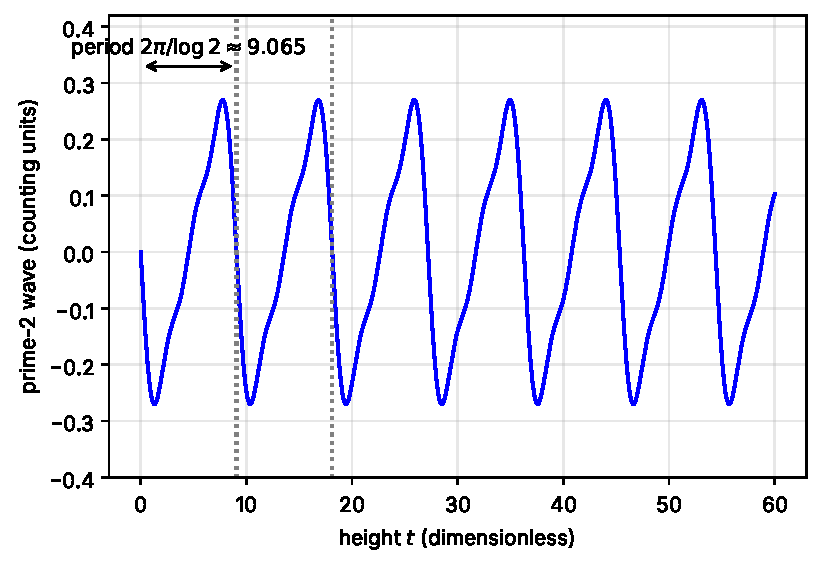
\includegraphics[width=0.85\linewidth]{figs/intro_prime2.pdf}
\caption{The prime-2 wave of \cref{eq:intro-re2} (running example RE2), plotted for $0 \le t \le 60$. Its period in $t$ is $2\pi/\log 2 \approx 9.065$ (two periods marked). In the paper's continuation probe (Sec.~III) a fitted potential is trained on a window of this wave and asked to continue it.}
\label{fig:intro-prime2}
\end{figure}

Adding the waves for $p = 2, 3, 5, 7, 11, 13$ gives a formula with no adjustable numbers in it at all. You solve "smooth curve plus waves $= n - \tfrac12$" for $t$ and get a prediction of the $n$-th zero. The paper calls this the \emph{arithmetic oracle} (paper Sec.~II~D, Eq.~(4)). It is not new mathematics: it is a truncation of the classical explicit formula connecting zeros and primes \cite{francaleclair,leclair}. But it predicts the zeros remarkably well, and it will serve as the yardstick that tells us how much predictable structure exists.

\begin{sample}{How many zeros fit in one prime-2 period?}
Near zero 500 the mean spacing is $1.292672$ (Sample Problem ``Measuring an error in mean spacings''). How many zeros, on average, lie within one period of the prime-2 wave there? What is the corresponding number near $t=50$, where \cref{eq:intro-gap} gives a mean spacing of $3.029288$?

\textbf{Step 1:} The period of the wave in $t$ is $2\pi/\log 2 = 6.2831853/0.6931472 = 9.064720$.

\textbf{Step 2:} The number of zeros per period near zero 500 is the period divided by the spacing: $9.064720/1.292672 = 7.012$.

\textbf{Step 3:} Near $t=50$: $9.064720/3.029288 = 2.992$.

\textbf{Answer:}
\[
\boxed{\text{about 7.0 zeros per period near zero 500; about 3.0 near } t=50}
\]
So even the slowest prime wave wiggles on a scale of a handful of zeros. The paper makes the same point in Sec.~V: the $p=2$ period of about 9 in $t$ is only about 6--7 levels at the heights it studies.
\end{sample}

\begin{beyond}
\textbf{What this chapter takes on trust.} The list of zeros (computed with the mpmath library, Chapter~\ref{ch:zeta}); the smooth counting curve \cref{eq:intro-Nsm} and the mean-spacing formula \cref{eq:intro-gap} (derived in Chapter~\ref{ch:counting-zeros}); the description of the wobble as a sum of prime waves (Chapter~\ref{ch:explicit-formula}, where we also explain that this sum is a heuristic approximation whose exact rigorous form is more delicate). Nothing in this chapter depends on any of these beyond their use as illustrations. Classic accounts are Edwards \cite{edwards} and Titchmarsh \cite{titchmarsh}.
\end{beyond}

\begin{checkpoint}
A friend says: ``The Riemann hypothesis was proved when computers found that billions of zeros lie on the line.'' What is wrong with this statement?
\end{checkpoint}
\checkanswer{Checking finitely many zeros, however many, does not prove a statement about infinitely many. The Riemann hypothesis remains an open conjecture; the numerical checks are evidence, not proof.}

\begin{keyideas}
\item The numbers $t_n$ are heights of nontrivial zeros $\rho_n = \tfrac12 + i t_n$ of the Riemann zeta function, a function built from the primes.
\item The Riemann hypothesis (all nontrivial zeros on the line $\tfrac12 + i t$) is open; all zeros used in the paper lie in the range where the line has been verified numerically.
\item The wobble of the zeros is approximately a sum of waves with frequencies $m\log p$ in $t$. The $p=2$ wave (RE2) has period $2\pi/\log 2 \approx 9.065$.
\item A truncated version of this sum, with no adjustable parameters, is the paper's arithmetic oracle (Eq.~(4)).
\end{keyideas}

%======================================================================
\section{Do the zeros look like energy levels?}\label{sec:intro-hp}
% DYK-BEGIN
\begin{didyouknow}{A Fateful Teatime}
In 1972 the number theorist Hugh Montgomery visited the Institute for Advanced Study in Princeton. Over afternoon tea, Sarvadaman Chowla introduced him to the physicist Freeman Dyson. Montgomery described his formula for how pairs of zeta zeros are spaced, and Dyson recognized it at once. It was the pair correlation of eigenvalues of large random complex Hermitian matrices, the kind of model physicists had built for the energy levels of heavy nuclei.
\end{didyouknow}
% DYK-END

\subsection{Allowed frequencies and allowed energies}

You already know a physical system with a discrete list of allowed values: a string fixed at both ends. It can vibrate only at frequencies $f_1, 2f_1, 3f_1, \ldots$, the harmonics \cite{hrw}. A plucked guitar string has a ``spectrum'' of equally spaced frequencies.

Quantum mechanics generalizes this. A particle trapped in a valley of potential energy $V(x)$ can only have certain energies $E_1 < E_2 < E_3 < \cdots$, called its \emph{energy levels} or its \emph{spectrum}. The reason is the same as for the string: the particle is described by a wave, and only waves that ``fit'' in the valley are allowed. You will learn this from scratch in Chapters~\ref{ch:schrodinger} and \ref{ch:bound-states}. The shape of the valley decides the levels. A box with vertical walls gives levels whose spacing grows with energy. A parabolic valley (a spring) gives equally spaced levels. For valleys of power-law shape, $V \propto \abs{x}^a$, walls rising more slowly than a parabola ($a < 2$) give levels whose spacing shrinks as energy grows, just like the zeros (Chapter~\ref{ch:bound-states} shows this; it is a semiclassical result, accurate for high levels).

\subsection{Level repulsion}

There is more to the resemblance than crowding. Look at \cref{fig:intro-barcode}. The top row shows the first 29 zeros as tick marks; the middle row shows 29 points thrown down independently at random over the same range; the bottom row shows 29 equally spaced ticks, like harmonics. The zeros are irregular, but not in the way the random points are irregular. Random points often land almost on top of each other. The zeros almost never do: small gaps are rare (a numerical observation, made over all the zeros computed). Physicists call this \emph{level repulsion}, and it is the hallmark of the energy levels of complicated quantum systems.

\begin{figure}[htbp]\centering
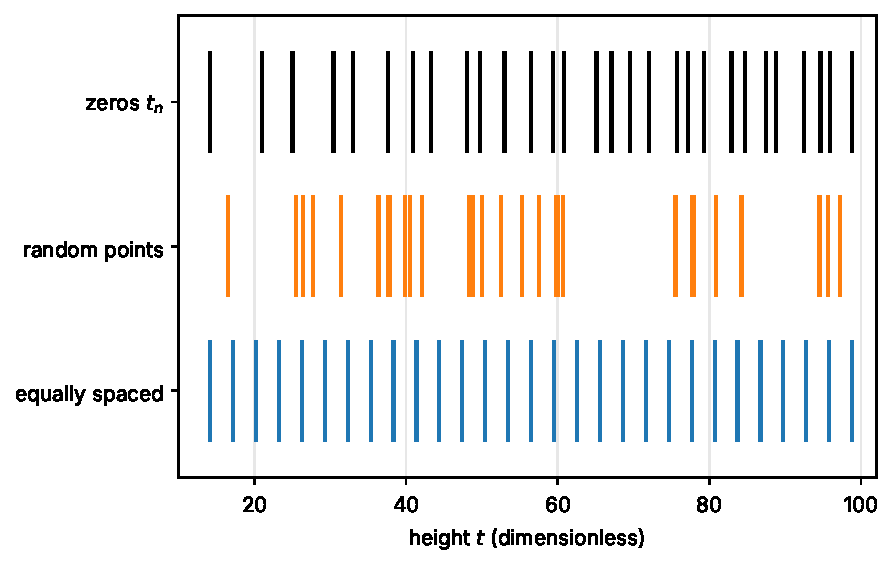
\includegraphics[width=0.85\linewidth]{figs/intro_barcode.pdf}
\caption{Top: the first 29 zero heights $t_1,\ldots,t_{29}$ (all zeros with $t \le 100$) as tick marks. Middle: 29 points placed independently at random over the same range (fixed seed), for comparison. Bottom: 29 equally spaced ticks spanning the same range, like the harmonics of a string. The zeros are irregular but avoid close pairs, unlike the random points.}
\label{fig:intro-barcode}
\end{figure}

This is not just an impression. Odlyzko's extensive computations \cite{odlyzko87} show numerically that the statistics of the gaps match those of the eigenvalues of large random matrices of a particular type, the Gaussian unitary ensemble (GUE). (A matrix is a square table of numbers; its eigenvalues are a list of characteristic numbers attached to it, which for the matrices of quantum mechanics are the energy levels; a random matrix has entries drawn at random. Chapters~\ref{ch:eigen} and \ref{ch:level-statistics} explain these ideas.) On the theoretical side, a theorem of Montgomery \cite{montgomery}, proved assuming the Riemann hypothesis, shows that the pair correlation of the zeros (how often two zeros lie a given distance apart) agrees with the GUE prediction, but only when tested with a restricted class of test functions. The full agreement, and in particular the agreement of the nearest-neighbor gap distribution, is a numerical observation, not a theorem. Fig.~2 of the paper shows this match for the first $10^4$ zeros. Chapter~\ref{ch:level-statistics} explains what these words mean and derives the curve plotted there.

\subsection{The Hilbert--P\'olya hope}

Put these hints together and you arrive at an idea attributed to Hilbert and P\'olya: perhaps the $t_n$ are exactly the energy levels of some quantum system. In mathematical language, perhaps they are the spectrum of a \emph{self-adjoint operator}. You will meet operators in Chapter~\ref{ch:schrodinger}; the important property of "self-adjoint" is that it forces every energy level to be an ordinary real number. If someone found a self-adjoint operator whose spectrum is exactly the set of heights $t_n$ (each nontrivial zero being written as $\tfrac12 + i t_n$), the realness of its energies would force every $t_n$ to be real, and that would put every zero on the line: the Riemann hypothesis would follow. No such operator is known; the idea is a conjecture. A second hint is that the wobble formula looks like the semiclassical formulas physicists use for chaotic quantum systems, with primes playing the role of closed classical orbits \cite{berrykeating99,schumayer}. Chapter~\ref{ch:hilbert-polya} tells this story.

\begin{pitfall}
The Hilbert--P\'olya idea is a \emph{conjecture}, a hope. No such operator is known. The GUE statistics are numerical observations and partial theorems; they show the zeros \emph{behave statistically} like energy levels of a certain class of systems, not that a specific system exists. Never read ``the zeros look like energy levels'' as ``the zeros are energy levels''.
\end{pitfall}

\subsection{Two programs: analytic and empirical}

Researchers have pursued the hope in two ways. The \emph{analytic program} tries to write down an operator from first principles and then show its spectrum is the list of zeros. The paper does not test this program and makes no claim against it (paper Sec.~I and Sec.~VI).

The \emph{empirical program} works backwards from the data. Wu and Sprung \cite{wusprung} built a smooth one-dimensional valley whose energy levels reproduce the \emph{smooth} part of the zeros, the positions $s_n$. Chapter~\ref{ch:wu-sprung} derives their construction; for now, picture a symmetric valley with its bottom at energy $V_0 = 3.10073\pi$, rising slowly on both sides, inside a box with hard walls at $x = \pm L$ (the paper's first scale uses $L = 44.883$; running example RE3). Then they added small fitted wiggles to the valley to reproduce the wobble too. Successors refined this \cite{vanzyl,slater,jaksch}. The implicit logic, in the paper's words, is that ``a potential reproducing many zeros accurately has captured something about the putative zeta operator'' (paper Sec.~I).

\subsection{Each level feels the valley near its turning points}

One piece of first-year physics will help you understand the paper's results. A ball rolling in a valley with total energy $E$ turns around at the points where the valley's height equals $E$: the turning points. A quantum particle in level $n$ is not a ball, but it behaves similarly in one way that matters here: its wave is most sensitive to the shape of the valley near its classical turning points (a semiclassical, approximate statement, made precise in Chapter~\ref{ch:wkb}). Low levels turn near the bottom of the valley, close to $x=0$; high levels turn far up the walls. So, roughly, \emph{position in the valley maps to level index}. If you change the valley near some position $x$, you mainly move the levels that turn near $x$. Chapter~\ref{ch:wkb} makes this precise.

\begin{checkpoint}
You raise the walls of the valley slightly, only near $x = \pm 25$, leaving the rest unchanged. Which levels move most: the lowest levels, the levels whose turning points are near $x = \pm 25$, or the highest levels?
\end{checkpoint}
\checkanswer{The levels whose classical turning points lie near $x=\pm25$. Their waves are most sensitive to the valley there. Levels that turn well inside never reach that region strongly, and levels that turn far outside are affected too, but less: by the classical analogy the particle moves fast there and spends little time in that region (Chapter~\ref{ch:wkb} makes this quantitative).}

\begin{keyideas}
\item A quantum particle in a potential valley has a discrete spectrum of energy levels, as a string has harmonics.
\item The zeros crowd together and show level repulsion, matching GUE statistics (paper Fig.~2); this is evidence of resemblance, not of a specific operator.
\item The Hilbert--P\'olya idea (zeros as the spectrum of a self-adjoint operator) is open.
\item The empirical program fits a potential, the Wu--Sprung background plus fitted wiggles, to the zeros.
\item Each level is most sensitive to the valley near its turning points, so position in the valley maps to level index.
\end{keyideas}

%======================================================================
\section{What it means to fit a model}\label{sec:intro-fitting}

\subsection{The ruler and the points}

Suppose you hang masses on a spring and record the stretch. You get five points on graph paper. You lay a ruler across them and draw a line that passes close to all of them. That line is a \emph{model}: a rule that turns an input (mass) into an output (stretch). The line has two adjustable numbers, its slope and its intercept. Adjustable numbers in a model are called \emph{parameters}, and choosing them to match data is called \emph{fitting}.

The differences between the data and the model at the data points are the \emph{residuals}; in this chapter we also call them errors. To summarize how well a model fits, we use the root mean square (rms) of the errors $e_1, \ldots, e_K$, where $K$ is simply how many errors there are:
\begin{equation}
\rms = \sqrt{\frac{e_1^2 + e_2^2 + \cdots + e_K^2}{K}} .
\label{eq:intro-rms}
\end{equation}
Read the name backwards to compute it: square each error, take the mean, take the square root. Squaring makes positive and negative errors count alike. The rms has the same units as the errors. (It is not the same as the standard deviation, which measures spread about the mean of a list; Chapter~\ref{ch:probability} explains the difference.)

\begin{sample}{Fitting with a ruler}
A student records five points $(x, y)$: $(0, 1.0)$, $(1, 2.9)$, $(2, 5.2)$, $(3, 6.9)$, $(4, 9.1)$. She draws the straight line through the first and last points. (a) Find its slope and intercept. (b) Find the residuals and their rms. (c) Predict $y$ at $x = 5$. Later she measures $y = 11.0$ at $x = 5$; what is the prediction error?

\textbf{Step 1: slope.} The line passes through $(0, 1.0)$ and $(4, 9.1)$, so its slope is $(9.1 - 1.0)/(4 - 0) = 8.1/4 = 2.025$.

\textbf{Step 2: intercept.} At $x=0$ the line passes through $y = 1.0$, so the intercept is $1.0$ and the line is $y = 1.0 + 2.025x$.

\textbf{Step 3: model values.} At $x = 1, 2, 3$ the line gives $3.025$, $5.050$, $7.075$; at $x=0$ and $4$ it reproduces the data exactly.

\textbf{Step 4: residuals (data minus model).} At $x=0,1,2,3,4$: $0$, $2.9-3.025 = -0.125$, $5.2 - 5.050 = +0.150$, $6.9 - 7.075 = -0.175$, $0$.

\textbf{Step 5: rms.} The squares are $0$, $0.015625$, $0.0225$, $0.030625$, $0$. Their sum is $0.06875$. Divide by $K = 5$: $0.01375$. The square root is $0.11726$.

\textbf{Step 6: prediction.} At $x = 5$: $1.0 + 2.025 \times 5 = 11.125$. The error against the later measurement is $11.125 - 11.0 = 0.125$.

\textbf{Answer:}
\[
\boxed{y = 1.0 + 2.025x,\quad \text{in-sample rms} = 0.117,\quad \text{prediction at } x=5: 11.125\ (\text{error } 0.125)}
\]
The prediction error is about the same size as the in-sample residuals. That is the signature of a model that has captured the trend.
\end{sample}

\subsection{More knobs: a curve through every point}

Now suppose instead of a ruler you use a flexible curve with as many knobs as there are data points. With five points you can always find a polynomial of degree 4, $y = a_0 + a_1x + a_2x^2 + a_3x^3 + a_4x^4$, which has five parameters, that passes \emph{exactly} through all five. Its in-sample rms is zero. Is it a better model?

\begin{sample}{The memorizing polynomial}
For the five points of the Sample Problem ``Fitting with a ruler'', the degree-4 polynomial through all of them is unique. (Two such polynomials would differ by a polynomial of degree at most 4 that vanishes at all five points; a nonzero polynomial of degree at most 4 has at most four roots, a fact from algebra taken on trust here and revisited with polynomial fitting in Chapter~\ref{ch:least-squares}; so the difference is zero.) Predict its value at $x = 5$ without finding its coefficients, using the fact that the fourth differences of a degree-4 polynomial at equally spaced points are constant.

\textbf{Step 1: first differences} (each value minus the previous one): $2.9-1.0 = 1.9$, $5.2 - 2.9 = 2.3$, $6.9 - 5.2 = 1.7$, $9.1 - 6.9 = 2.2$.

\textbf{Step 2: second differences:} $2.3 - 1.9 = 0.4$, $1.7 - 2.3 = -0.6$, $2.2 - 1.7 = 0.5$.

\textbf{Step 3: third differences:} $-0.6 - 0.4 = -1.0$, $0.5 - (-0.6) = 1.1$.

\textbf{Step 4: fourth difference:} $1.1 - (-1.0) = 2.1$. For a degree-4 polynomial this stays $2.1$ forever. (Why: for a power $x^k$, the binomial expansion gives $(x+1)^k - x^k = k x^{k-1} + (\text{terms with lower powers of } x)$, so taking differences at points spaced by 1 turns a polynomial of degree $k$ into one of degree $k-1$. Four differencings turn a degree-4 polynomial into a polynomial of degree 0, a constant. For example, the values of $x^4$ at $x = 0,1,2,3,4$ are $0, 1, 16, 81, 256$; their first differences are $1, 15, 65, 175$, the second $14, 50, 110$, the third $36, 60$, and the fourth $24$, and every further fourth difference is also $24$. Problem 23 asks you to confirm the prediction numerically.)

\textbf{Step 5: extend the table one column to the right.} New third difference: $1.1 + 2.1 = 3.2$. New second difference: $0.5 + 3.2 = 3.7$. New first difference: $2.2 + 3.7 = 5.9$. New value: $9.1 + 5.9 = 15.0$.

\textbf{Answer:}
\[
\boxed{\text{polynomial predicts } y(5) = 15.0;\ \text{error } 4.0 \text{ against the measured } 11.0}
\]
Its in-sample error is zero, yet its prediction error is 32 times that of the ruler line ($4.0/0.125 = 32$). The polynomial bent itself to the noise in the five points. \Cref{fig:intro-memorize} shows the picture.
\end{sample}

\begin{figure}[htbp]\centering
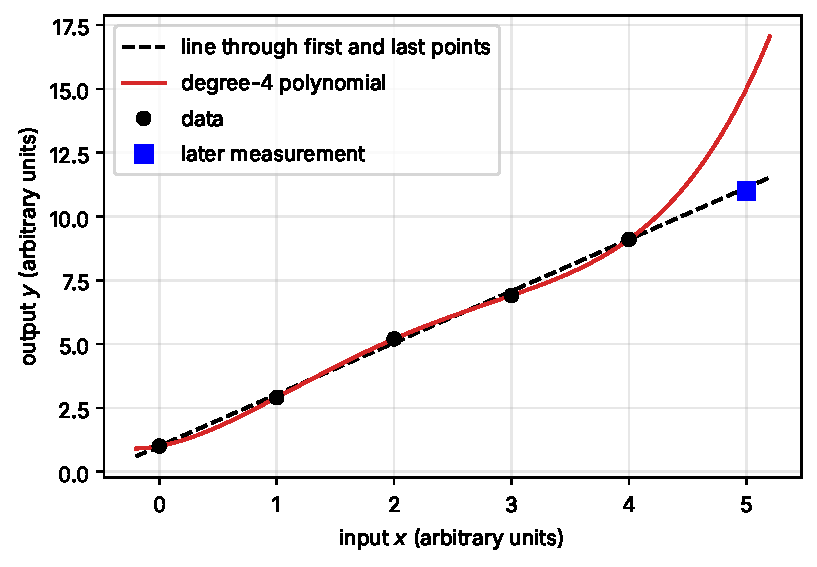
\includegraphics[width=0.85\linewidth]{figs/intro_memorize.pdf}
\caption{Five measured points (dots) fitted by the straight line through the first and last points (dashed; in-sample rms $0.117$) and by the degree-4 polynomial through all five (solid; in-sample rms $0$). The later measurement at $x = 5$ (square, $y = 11.0$) is predicted to within $0.125$ by the line and missed by $4.0$ by the polynomial, which predicts $15.0$.}
\label{fig:intro-memorize}
\end{figure}

This is the simplest picture of memorization, and you will see a fuller version (running example RE4, a polynomial fitted to noisy samples of $\sin t$) in Chapters~\ref{ch:least-squares} and \ref{ch:generalization}. The lesson: \emph{when a model has enough knobs to pass through every data point, a perfect fit tells you nothing about whether it has learned the rule.}

\subsection{Fitting a potential}

The paper fits something much more elaborate than a line, but the idea is the same. The model is the Wu--Sprung valley plus a correction $\delta V(x)$ (``delta V'') built from $M$ smooth wiggles, each multiplied by an adjustable coefficient. The default wiggles are cosines across the box. The $M$ coefficients are the knobs. For each setting of the knobs, a computer finds the energy levels of the corrected valley (Chapter~\ref{ch:finite-differences}), and an optimizer adjusts the knobs to make the levels match the zeros (Chapter~\ref{ch:fitting}). The paper uses $M$ between 200 and 900, fitted to a few hundred zeros. With 900 knobs and 500 zeros there are more knobs than data, a situation even more permissive than the degree-4 polynomial through five points, where knobs and data were equal in number. (Because the levels depend on the knobs in a nonlinear way, counting knobs alone does not guarantee an exact fit; in practice the paper's fits come very close, Finding 1 of \cref{sec:intro-result}.)

\begin{checkpoint}
A model with 400 adjustable coefficients reproduces 400 data points with an rms error of $10^{-4}$. A colleague says this proves the model has found the law behind the data. What single additional test would you ask for?
\end{checkpoint}
\checkanswer{Ask how well it predicts data points it was not fitted to (held-out data), compared with a simple baseline. With as many knobs as data points, a near-perfect in-sample fit is expected whether or not the model has found the law.}

\begin{keyideas}
\item A model is a rule with adjustable parameters; fitting chooses them to match data; residuals are data minus model.
\item The rms error \cref{eq:intro-rms} summarizes the size of a list of errors.
\item A model with as many parameters as data points can fit exactly while predicting badly.
\item The paper's model is the Wu--Sprung potential plus a correction with $M$ fitted coefficients.
\end{keyideas}

%======================================================================
\section{Memorizing versus predicting}\label{sec:intro-memorize}

\subsection{Two students}

Two students prepare for an exam. The first obtains last year's paper with its answers and memorizes them. The second works through the course and learns how to solve the problems. On last year's paper, both score 100\%. The difference only appears on a new exam.

\begin{sample}{The memorizing student}
A multiple-choice exam has 20 questions, each with 4 options. Student A has memorized the answers to last year's 20 questions and nothing else. This year's exam reuses 4 of last year's questions; on the other 16, student A guesses at random. Student B understands the material and answers 85\% of any set of questions correctly. Find each student's expected score on this year's exam, and on last year's exam.

\textbf{Step 1: last year's exam.} A knows all 20 answers: score 20/20, that is 100\%. B gets 85\% of 20, which is 17, so 85\%.

\textbf{Step 2: A on the repeated questions.} A answers all 4 correctly.

\textbf{Step 3: A on the new questions.} A random guess among 4 options is right with probability $1/4$, so on average A gets $16 \times \tfrac14 = 4$ of the 16 right.

\textbf{Step 4: A's expected total:} $4 + 4 = 8$ out of 20, which is 40\%.

\textbf{Step 5: B's expected total:} $0.85 \times 20 = 17$ out of 20, that is 85\%, the same as last year.

\textbf{Answer:}
\[
\boxed{\text{Last year: A } 100\%,\ \text{B } 85\%.\qquad \text{This year: A } 40\%,\ \text{B } 85\%.}
\]
On the old paper A looks better than B. Only the new paper reveals which student learned the rule. And A's new score should be compared with what pure guessing would give: $20 \times \tfrac14 = 5$ out of 20, that is 25\%. A beats guessing only because of the 4 repeated questions. Those repeats are a \emph{leak} of training data into the test. A clean held-out test contains none of the training questions; on such a test A would expect exactly $20\times\tfrac14 = 5$ out of 20, the guessing (null) score, while B would still expect 17. The clean case is the one the paper sets up for the zeros.
\end{sample}

Every element of this story has a name. Last year's paper is the \emph{training data}: the data the model is fitted to. This year's new questions are the \emph{held-out data} (also called test data, or \emph{out-of-sample}, OOS, data): data deliberately kept away from the fitting and used only to score the model. The score on training data is the \emph{in-sample} score. Pure guessing is a \emph{null model}: the simplest possible prediction, against which any claim of skill must be measured.

\subsection{Training and held-out zeros}

In the paper the training data are the first $n_{\rm fit}$ zeros, for example zeros 1--400. The held-out data are the next ones, for example zeros 401--500, which is the paper's principal holdout and the fifth running example of the book (RE5). The model is fitted to zeros 1--400 only; then its predicted levels 401--500 are compared with the true zeros. Neither the fitted potential's prediction nor that of the explicit formula (which has nothing fitted at all) uses any zero past the boundary (paper Fig.~1 caption).

What is the null model here? It is ``no fluctuation'': predict that each zero sits exactly at its smooth position $s_n$, or, for the potential, that its levels are those of the unperturbed Wu--Sprung valley. The paper finds that these two nulls give the same error on zeros 401--500, an rms of $0.263$ mean spacings (paper Sec.~II~C). The two are different objects (an eigenvalue spectrum and the solution of a counting equation); it is their numerical coincidence on this holdout (both $0.2631$) that lets the paper use one baseline. In other words, the typical fluctuation of those zeros is about a quarter of a spacing, and a model must beat $0.263$ to show any skill.

\begin{figure}[htbp]\centering
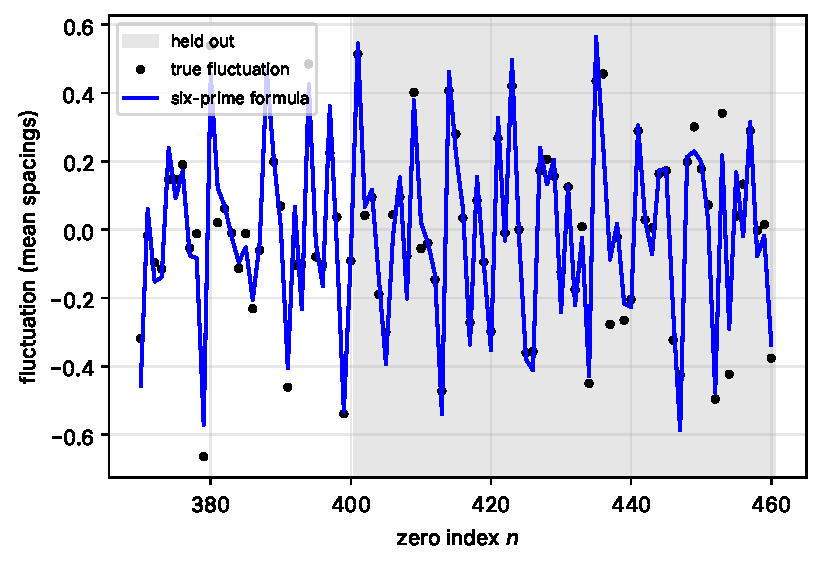
\includegraphics[width=0.85\linewidth]{figs/intro_trainhold.pdf}
\caption{True fluctuations (dots, in mean spacings) of zeros 370--460, and the prediction of the six-prime explicit formula of paper Eq.~(4) (line), which has no fitted parameters. The shaded region is held out: in the paper's experiment, models are fitted only to zeros 1--400. The paper reports held-out rms $0.074$ and correlation $+0.96$ for this formula on zeros 401--500 (paper Table~V). The plotted window 370--460 matches paper Fig.~1; the quoted scores refer to the whole holdout 401--500. This figure omits the fitted operator shown in paper Fig.~1.}
\label{fig:intro-trainhold}
\end{figure}

\subsection{Two scores: rms and correlation}

The paper reports two numbers for each prediction. The first is the rms error \cref{eq:intro-rms} in mean spacings. The second is the \emph{correlation} between predicted and true fluctuations, a number between $-1$ and $+1$ defined precisely in Chapter~\ref{ch:probability}. For now: correlation $+1$ means the prediction goes up exactly where the truth goes up and down where it goes down (the shapes agree perfectly, whatever the size); $0$ means no relation; $-1$ means the shapes are mirror images. The two scores measure different things, as the next example shows.

\begin{sample}{Why both rms and correlation are reported}
The true fluctuations of five zeros are $0.2, -0.3, 0.1, 0.4, -0.4$ (in mean spacings). Compare three predictions: (a) the null, predicting $0$ for every zero; (b) a prediction equal to half the truth, $0.1, -0.15, 0.05, 0.2, -0.2$; (c) a prediction equal to minus half the truth. Give each one's rms error and say what its correlation with the truth is.

\textbf{Step 1: the null.} Its errors are the truth itself. Squares: $0.04, 0.09, 0.01, 0.16, 0.16$; sum $0.46$; mean $0.092$; rms $\sqrt{0.092} = 0.3033$. Its correlation is undefined: correlation is defined only for predictions that vary from zero to zero, and a constant prediction has no shape. So no correlation is reported for the null; it carries no information about the shape.

\textbf{Step 2: half the truth.} Each error is truth minus prediction $= 0.5\times$ truth. Squaring multiplies every square by $0.25$, so the mean square is $0.25 \times 0.092 = 0.023$ and the rms is $0.5 \times 0.3033 = 0.1517$. The prediction has exactly the shape of the truth, so the correlation is $+1$.

\textbf{Step 3: minus half the truth.} Each error is truth $-(-0.5\times$ truth$) = 1.5\times$ truth. The rms is $1.5\times0.3033 = 0.4550$. The shape is the mirror image, so the correlation is $-1$.

\textbf{Answer:}
\[
\boxed{\text{rms: null } 0.303,\ \ \text{(b) } 0.152 \ (\text{corr} +1),\ \ \text{(c) } 0.455\ (\text{corr} -1)}
\]
A prediction with the right shape but the wrong size can still have a sizeable rms; a prediction with the wrong shape can be worse than the null. That is why the paper always gives the pair ``rms / corr'', and why, in this book, we call a result skillful only if the rms is below the null \emph{and} the correlation is reproducibly positive, which is how the paper reads its own tables.
\end{sample}

\begin{checkpoint}
A fitted model's held-out rms is $0.30$ where the null is $0.263$, and its correlation with the truth is $-0.02$. Has it learned anything that transfers to the held-out zeros?
\end{checkpoint}
\checkanswer{No. It does worse than predicting no fluctuation at all, and its output has no relation to the shape of the truth. Whatever it learned in-sample does not transfer.}

\begin{keyideas}
\item Training data are used for fitting; held-out (out-of-sample) data are used only for scoring.
\item Every claim of skill is relative to a null model; for the zeros the null is "no fluctuation", with rms $0.263$ on zeros 401--500 (RE5).
\item rms measures size of error; correlation measures agreement of shape. Both are needed.
\item Memorizing gives a perfect training score and no held-out skill; learning the rule gives similar scores on both.
\end{keyideas}

%======================================================================
\section{The paper's result in one page}\label{sec:intro-result}

We can now say in plain words what the paper \cite{soniR1} did and found. Its title is the summary: ``Fitted potentials on the Wu--Sprung background memorize the Riemann zeros while the explicit formula predicts them.''

\textbf{The question.} The empirical Hilbert--P\'olya program judges a fitted potential by how well its levels match the zeros it was fitted to. The paper applies the test that program had lacked: does the fitted potential predict zeros it was not shown? The scope is deliberately narrow: fitted corrections on the Wu--Sprung background, in three families of wiggles (cosines; Chebyshev polynomials, a standard family of polynomials; and local ``hat'' functions, little triangular bumps; all defined in Chapter~\ref{ch:fitting}), with one fitting method, in two box sizes that the paper calls scale~1 ($L = 44.883$, first 500 levels scored) and scale~2 ($L = 59.957$, first 1000 levels). Other backgrounds and other families are not tested, and analytic operator proposals are not touched (paper Sec.~I).

\textbf{Finding 1: fitting is easy.} With a few hundred coefficients the fitted potential reproduces its training zeros very closely; on all 500 zeros of the first scale it reaches rms below $10^{-4}$ spacings at $M = 900$ (paper Sec.~III).

\textbf{Finding 2: transfer is nil.} In every configuration examined (two scales, several splits, three bases, a range of $M$, regularization, that is a penalty that discourages large coefficients (Chapter~\ref{ch:least-squares}), and optimizer restarts), the fitted potentials show no reproducible held-out skill: their held-out rms never improves on the null, and no reproducible positive correlation with the truth appears (paper Tables~I--III). One Chebyshev row is marginal, and the paper reports it as such: rms $0.291$ with correlation $+0.18$, whose bootstrap intervals include the null and reach down to zero; a small positive correlation for that row is not excluded (paper Table~II). For the principal case (fit zeros 1--400 with $M=400$ cosines, score zeros 401--500) the in-sample rms is $0.137$ but the held-out rms is $0.369$, worse than the null $0.263$, with correlation $-0.07$ (paper Table~I).

\textbf{Finding 3: the fit does as well on fakes as on the real zeros.} In the principal configuration (scale~1, $M = 400$, zeros 1--400, ten fake draws of each kind), refitted to shuffled versions of the fluctuations, to phase-randomized fakes \cite{theiler} and to amplitude-adjusted fakes \cite{schreiber} (the last two keep the overall wiggliness, the power spectrum, but have no arithmetic content), the fit reaches the same in-sample accuracy as on the real zeros (paper Sec.~III). Its in-sample success measures its capacity, not its understanding.

\textbf{Finding 4: it did not continue even one prime wave.} Trained on levels 1--400 with a target that is nothing but the prime-2 wave (RE2), it reproduces the wave in-sample (rms $0.056$, correlation $+0.95$) and, under the fitting protocol used, did not continue it on levels 401--500 (held-out correlation $+0.07$, rms worse than predicting zero fluctuation) (paper Sec.~III, "Arithmetic-continuation probe"). The paper calls this ``the memorization mechanism exhibited in isolation''.

\textbf{Finding 5: the arithmetic predicts.} The explicit formula truncated to six primes, with zero fitted parameters, scores rms $0.074$ and correlation $+0.96$ on zeros 401--500; with 25 primes, $0.043$ and $+0.99$; the skill hardly changes up to zero $10^4$ (paper Table~V, Fig.~1).

\textbf{Finding 6: the obstacle is the parametrization, not the parameter count.} A generic 900-coefficient sum of sinusoids also fails to beat the null, but a fitted model told only that the fluctuation is a sum of a \emph{few} sinusoids finds, from 400 zeros, frequencies at logarithms of primes and prime powers, and predicts zeros 401--500 at $0.034$ with correlation $+0.99$ (paper Sec.~IV, Table~IV). That the zeros' wobble is concentrated at those frequencies is classical \cite{landau,gonek}; the paper uses it as a control, not as a new result.

\textbf{A side lesson.} A separate investigation of complex-valued (non-Hermitian) corrections (``Hermitian'' is the property that guarantees real energies, Chapter~\ref{ch:schrodinger}; these corrections lack it, Chapter~\ref{ch:non-hermitian}) found an apparently meaningful in-sample ``floor'' that turned out to be manufactured by an approximation used outside its range of validity and by a numerically dead parameter feeding on round-off noise; exact computation dissolved it (paper Sec.~V).

\textbf{The proposal.} Any future claim that a fitted operator ``captures'' the zeros should come with held-out scores against its own null, including a split within one height range; scoring of the actual operator; evidence of robustness to regularization and restarts; and refits to shuffled and phase-randomized targets (paper Sec.~VI).

The paper keeps its explanation of \emph{why} the fits fail modest: it offers a heuristic reading (the potential addresses levels locally through their turning points, while the fluctuation is a sum of long-range waves in $t$) and states that deriving the memorization result is an open problem.

\begin{sample}{Reading headline numbers against the null}
Using the paper's numbers, express (a) the operator's held-out rms for the principal case and (b) the six-prime oracle's held-out rms on the same holdout as multiples of the null $0.263$.

\textbf{Step 1:} Operator, paper Table~I (scale 1, fit zeros 1--400, $M=400$): $0.369/0.263 = 1.403$.

\textbf{Step 2:} Six-prime oracle, paper Table~V (holdout 401--500): $0.074/0.263 = 0.281$.

\textbf{Step 3:} Interpret. The operator's error is about $40\%$ larger than predicting no fluctuation. The oracle's error is about $28\%$ of the null, a reduction of $1 - 0.281 = 0.719$, about $72\%$.

\textbf{Answer:}
\[
\boxed{\text{operator: } 1.40\times\text{null (worse)};\qquad \text{six-prime oracle: } 0.28\times\text{null (72\% better)}}
\]
\end{sample}

\begin{checkpoint}
The arithmetic oracle ``is not a fair machine-learning competitor'' (paper Sec.~IV). Why not, and what is its role then?
\end{checkpoint}
\checkanswer{It is handed the correct functional form (waves at frequencies $m\log p$) rather than learning anything. Its role is informational: it proves that transferable, predictable structure about unseen zeros exists, and it measures how much of it simple arithmetic captures.}

\begin{keyideas}
\item The paper tests fitted Wu--Sprung potentials by held-out prediction. They fit their training zeros closely and predict nothing beyond the null.
\item The fits succeed equally on shuffled and phase-randomized fakes, and did not, under the fitting protocol used, continue a single prime wave.
\item The truncated explicit formula, with zero fitted parameters, predicts held-out zeros with correlation up to $+0.99$ through zero $10^4$.
\item A fitted model with only a sparsity prior in frequency (the assumption that only a few frequencies are present) recovers the prime frequencies; the obstacle, for the families and fitting protocol tested, is the potential as parametrization rather than the number of parameters.
\item The explanation of the failure is heuristic; the scope is limited to the families tested.
\end{keyideas}

%======================================================================
\section{A road map of the book}\label{sec:intro-roadmap}
% DYK-BEGIN
\begin{didyouknow}{Eight Pages That Changed Mathematics}
Riemann's famous 1859 paper, \emph{On the Number of Primes Less Than a Given Magnitude}, was written on his election to the Berlin Academy and runs only about eight pages. It was his only paper on number theory. Yet it introduced the zeta function on the complex plane, the explicit formula linking zeros to primes, and the Riemann hypothesis itself.
\end{didyouknow}
% DYK-END

To read the paper line by line you need tools from several fields. The book is organized in six parts (\cref{fig:intro-roadmap}).

\textbf{Part I, Mathematical foundations} (Chapters~\ref{ch:complex}--\ref{ch:least-squares}): complex numbers and the exponential; series and infinite products; approximation, asymptotics and root finding; Fourier series; the Fourier transform and the periodogram; vectors and matrices; eigenvalues; least squares, the singular value decomposition and regularization.

\textbf{Part II, Quantum mechanics of a particle on a line} (Chapters~\ref{ch:schrodinger}--\ref{ch:non-hermitian}): wavefunctions and the Schr\"odinger equation; bound states; the semiclassical (WKB) approximation and level counting; perturbation theory; complex potentials and PT symmetry.

\textbf{Part III, Primes and the zeta function} (Chapters~\ref{ch:primes}--\ref{ch:explicit-formula}): the primes; the zeta function; counting the zeros; the explicit formula.

\textbf{Part IV, Spectra, randomness and operators} (Chapters~\ref{ch:probability}--\ref{ch:wu-sprung}): probability and statistics; level statistics and random matrices; the Hilbert--P\'olya dream; the Wu--Sprung construction.

\textbf{Part V, Computation, fitting and generalization} (Chapters~\ref{ch:finite-differences}--\ref{ch:sparse-frequency}): solving the Schr\"odinger equation on a computer; fitting a potential to a spectrum; memorization and generalization; uncertainty and controls; learning frequencies from data.

\textbf{Part VI, The paper, section by section} (Chapters~\ref{ch:paper-setup}--\ref{ch:paper-critique}): five chapters that teach no new mathematics but read the paper in order, rerun its key computations at small scale, and weigh its strengths and limits.

\begin{figure}[htbp]\centering
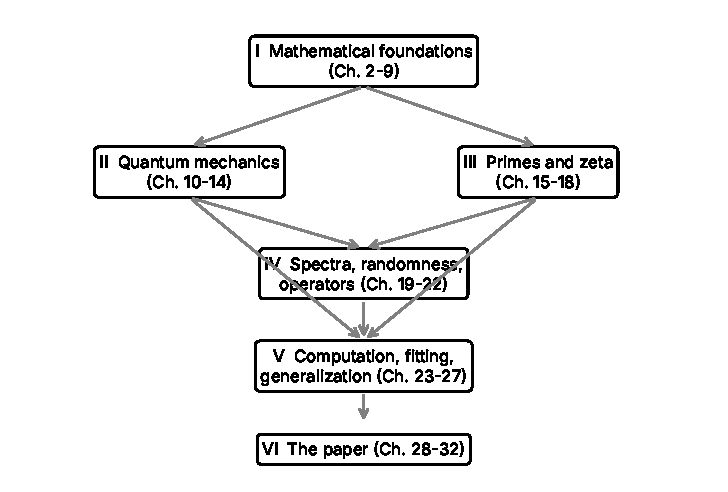
\includegraphics[width=0.85\linewidth]{figs/intro_roadmap.pdf}
\caption{Dependency diagram of the six parts of the book. An arrow from one part to another means the second uses tools from the first. Part I underlies everything; Parts II and III can be read in either order; Part VI uses all earlier parts.}
\label{fig:intro-roadmap}
\end{figure}

If you are mainly interested in the physics, Parts I and II, then Chapters~\ref{ch:counting-zeros}, \ref{ch:hilbert-polya} and \ref{ch:wu-sprung}, give the quantum side. If you are mainly interested in the data science, Chapters~\ref{ch:least-squares}, \ref{ch:probability} and Part V give the fitting and testing side. To read the paper fully you need all of it.

\begin{keyideas}
\item Six parts: mathematics, quantum mechanics, number theory, spectra and statistics, computation and fitting, and the paper itself.
\item Part I underlies everything; Part VI uses everything.
\end{keyideas}

%======================================================================
\section{How to use this book}\label{sec:intro-howto}

\textbf{Sample Problems} are fully worked examples, with every step numbered and the answer boxed. Cover the solution and try each one first.

\textbf{Checkpoints} are quick questions to test understanding; the answer follows immediately.

\textbf{Pitfalls} warn of common mistakes. \textbf{Beyond} boxes say exactly what is being taken on trust and where the proof can be found.

\textbf{Status labels.} Mathematics and science mix statements of very different strength. We label them consistently: a \emph{theorem} is proved (in the book or, if the proof is beyond us, in a cited source, and we say which); a \emph{heuristic} or \emph{approximate} statement holds under stated conditions; a \emph{conjecture} is open (the Riemann hypothesis and the Hilbert--P\'olya idea are conjectures); a \emph{numerical observation} is something seen in computations, which may or may not hold beyond them.

\textbf{Problems} at the end of each chapter are graded: level 1 problems check that you can use the ideas directly; level 2 problems require combining ideas; level 3 problems are harder or open-ended. Several problems in every chapter use the paper's own numbers and methods, and several are computational.

\textbf{Code.} Computational problems use Python with the numpy library and the book's companion library \texttt{qmnt}, which computes zeros, smooth zeros, the explicit-formula oracle, and the potentials and spectra of the paper. Appendix~A teaches all the Python you need, starting from nothing. The listing in \cref{sec:intro-numbers} is a typical example: a few lines that compute something you can check by hand.

\textbf{Reproducibility.} The paper's code and data are archived publicly \cite{zenodo}. In Part VI you will rerun parts of the paper's pipeline at small scale. The habit we want you to form is the one the paper itself argues for: before believing a number, see how it was computed and whether it can be recomputed.

\begin{keyideas}
\item Work the Sample Problems yourself before reading the solutions; use Checkpoints to check understanding.
\item Watch the status of every statement: theorem, heuristic, conjecture, or numerical observation.
\item Appendix~A teaches the Python used throughout.
\end{keyideas}

%======================================================================
\section{Paper connection}\label{sec:intro-paper}

This chapter prepares you to read the opening of the paper \cite{soniR1}. Here is what each part corresponds to, using the R1 numbering.

\textbf{Title and abstract.} The abstract contains the whole argument in compressed form. You can now decode most of its phrases: ``empirical Hilbert--P\'olya constructions'' (\cref{sec:intro-hp}); ``fit quantum Hamiltonians to the nontrivial Riemann zeros'' (\cref{sec:intro-fitting}; a Hamiltonian is the energy operator of a quantum system, Chapter~\ref{ch:schrodinger}); ``out-of-sample prediction'' (\cref{sec:intro-memorize}); ``up to 900 fitted coefficients, in cosine, Chebyshev, and local piecewise-linear bases'' (the three families of wiggles); ``relative to the unfitted potential'' (the null); ``shuffled and phase-randomized surrogate targets'' (Finding 3 of \cref{sec:intro-result}); ``a pure prime-2 explicit-formula oscillation'' (RE2, \cref{eq:intro-re2}); ``with zero fitted parameters predicts held-out zeros with correlation up to $+0.99$ through zero $10^4$'' (Finding 5). Chapter~\ref{ch:paper-setup} unpacks the abstract sentence by sentence.

\textbf{Sec.~I, first paragraph.} The definition $\rho_n = \tfrac12 + i t_n$ is our \cref{eq:intro-rho}. The phrase ``the spectrum of a self-adjoint operator'' is the Hilbert--P\'olya idea (\cref{sec:intro-hp}). The two strands of circumstantial evidence (GUE statistics \cite{montgomery,odlyzko87} and the trace-formula analogy \cite{berrykeating99,schumayer}), together with the continuing stream of explicit operator proposals, are the subjects of Chapters~\ref{ch:level-statistics} and \ref{ch:hilbert-polya}.

\textbf{Sec.~I, second paragraph.} The empirical program of Wu and Sprung \cite{wusprung} and successors, and its ``implicit logic'', are summarized in \cref{sec:intro-hp}. The scope statement (only fluctuation potentials on the Wu--Sprung background, three bases; no claim against analytic constructions; ``capture'' means predictive transfer measured by rms and correlation relative to the smooth baseline) is the honest boundary of every result. Notice also the sentence ``The novelty claimed is likewise not the explicit formula'': the paper claims novelty only for the controlled out-of-sample comparison.

\textbf{Sec.~I, third paragraph, and Fig.~1.} The summary of findings is our \cref{sec:intro-result}. Fig.~1 shows zeros 370--460 after a fit on zeros 1--400 at scale 1 with $M=400$; past the boundary the fitted operator's held-out correlation is $-0.07$ and the six-prime formula's is $+0.96$. Our \cref{fig:intro-trainhold} reproduces the true fluctuations and the six-prime prediction (not the operator, which needs Chapter~\ref{ch:fitting}).

\textbf{Sec.~I~A, Relation to prior work.} Its four strands are: (a) inverse-spectral fits \cite{wusprung,vanzyl,slater,jaksch}, which the paper says have been evaluated mainly by agreement with their own training zeros, a statement it supports by a citation-graph audit recorded in Appendix~A; (b) explicit formulas for the $n$-th zero \cite{francaleclair,leclair}, including Connes's prime-only construction \cite{connes26}, all on the arithmetic side of the comparison; (c) machine learning on zeros and arithmetic data; (d) operator proposals, which are not the target. Chapters~\ref{ch:hilbert-polya}, \ref{ch:wu-sprung} and \ref{ch:paper-setup} return to these. The Lambert-$W$ function mentioned in strand (b) is introduced in Chapter~\ref{ch:asymptotics}.

\textbf{Numbers you have already met.} Paper Eq.~(1) is our \cref{eq:intro-Nsm}; ``All errors below are quoted in units of the local mean spacing $\gap_n = ds_n/dn$'' (paper Sec.~II~A) is the convention of the Sample Problem ``Measuring an error in mean spacings''. The null $0.263$ on zeros 401--500 comes from paper Sec.~II~C and Tables~I and V. The headline rows used in the Sample Problem ``Reading headline numbers against the null'' are from paper Table~I (operator, $0.369/-0.07$) and Table~V (six primes, $0.074/+0.96$). The prime-2 period of about 9 in $t$ and ``6--7 levels'' appear in paper Sec.~V. Our \cref{fig:intro-barcode} illustrates qualitatively, with 29 zeros, the level repulsion that paper Fig.~2 shows quantitatively as a spacing histogram of the first $10^4$ zeros; Chapter~\ref{ch:level-statistics} explains that histogram.

\textbf{Sec.~II~F, Use of artificial intelligence.} The paper discloses that its computations, analysis and drafting were carried out with substantial assistance from a large language model, and that every reported number is regenerated by an archived scripted pipeline \cite{zenodo}. We note this neutrally here; Chapters~\ref{ch:paper-setup} and \ref{ch:paper-critique} discuss why such disclosures and reproducibility records matter.

%======================================================================
\section{Summary}\label{sec:intro-summary}

\begin{itemize}
\item The data are the heights $t_n$ of the nontrivial zeros $\rho_n = \tfrac12 + i t_n$ of the Riemann zeta function, \cref{eq:intro-rho}; the first ten (RE1) are in \cref{tab:intro-first10}.
\item The counting staircase $N(T)$, \cref{eq:intro-NT}, follows the smooth curve $\Nsm(T)$, \cref{eq:intro-Nsm} (paper Eq.~(1)); for example $N(100) = 29$ and $\Nsm(100) \approx 29.00$.
\item The local mean spacing is about $2\pi/\log(t/2\pi)$, \cref{eq:intro-gap}: about $1.29$ near zero 500. Errors are measured in these units.
\item The wobble of the zeros is approximately a sum of prime waves with frequencies $m\log p$; the $p=2$ wave (RE2, \cref{eq:intro-re2}) has period $2\pi/\log 2 \approx 9.065$.
\item The zeros resemble quantum energy levels (crowding, level repulsion, GUE statistics). The Riemann hypothesis and the Hilbert--P\'olya idea are open.
\item Fitting chooses parameters to match data; the rms \cref{eq:intro-rms} summarizes errors. A model with as many parameters as data can fit perfectly and predict badly (\cref{fig:intro-memorize}).
\item Skill is measured on held-out data, against a null model, with both rms and correlation. For zeros 401--500 (RE5) the null rms is $0.263$.
\item The paper's result: fitted Wu--Sprung potentials memorize (held-out rms $0.369$, correlation $-0.07$ in the principal case) while the six-prime explicit formula predicts ($0.074$, $+0.96$) with no fitted parameters; a sparsity prior in frequency suffices to learn the arithmetic structure.
\end{itemize}

%======================================================================
\section{Problems}\label{sec:intro-problems}

\begin{problemlist}
\prob{1}{In your own words, explain the difference between a model that memorizes its data and one that predicts. Give an everyday example of each that is not in this chapter.}

\prob{1}{Using \cref{tab:intro-first10}, compute the spacing between the ninth and tenth zeros directly from their heights, and say whether it is larger or smaller than the average spacing among the first ten zeros.}

\prob{1}{Near $t = 50$ the mean spacing from \cref{eq:intro-gap} is $3.029288$. A prediction misses a zero near $t=50$ by $0.6$ in $t$. Express the error in mean spacings.}

\prob{1}{Which of the following statements are correct? (a) The Riemann hypothesis has been proved. (b) Every zero used in the paper has been verified to lie on the line $\tfrac12 + it$. (c) A self-adjoint operator whose spectrum is the $t_n$ is known. (d) The gap statistics of the zeros match those of GUE random matrices numerically.}

\prob{2}{A student records the points $(0, 2.0)$, $(1, 3.4)$, $(2, 5.1)$, $(3, 6.4)$ and draws the line through the first and last. Find its slope, the residuals at $x = 1$ and $x=2$, and its prediction at $x=4$.}

\prob{2}{From paper Table~V, the null on zeros 401--500 is $0.263$, the six-prime oracle scores $0.074$, and the 25-prime oracle $0.043$. From paper Table~IV, the sparse frequency model C2 scores $0.034$. Express each of the three as a percentage reduction from the null.}

\prob{2}{From paper Table~I (scale 1, fit 1--400), the unregularized $M=400$ row has OOS rms $0.369$ and the ridge $\mu = 0.3$ row has $0.265$; the null is $0.263$. By what percentage is each worse than the null? What does the second number suggest regularization does?}

\prob{2}{A student memorizes the answers to 30 past questions. A new exam has 25 multiple-choice questions with 5 options each, of which 5 are past questions. Find the student's expected percentage score if she guesses on the rest, and compare it with the score from guessing everything.}

\prob{1}{The paper's largest cosine fit on the first scale uses $M = 900$ coefficients for 500 zeros. How many coefficients per zero is that? How many coefficients per training zero does the principal $M=400$, zeros 1--400 fit use? How many fitted parameters does the six-prime oracle have?}

\prob{2}{The errors of a prediction on four zeros are $0.3, -0.1, 0.0, -0.2$ mean spacings. Find the rms error.}

\prob{2}{Find the periods in $t$ of the second ($m=2$) and third ($m=3$) terms of the prime-2 wave \cref{eq:intro-re2}, and explain why the sum of all three terms has period $2\pi/\log 2$.}

\prob{3}{Suppose the true fluctuations have rms $R$ and a prediction equals $a$ times the truth for some number $a$. (a) Show the rms error is $\abs{1-a}\,R$. (b) Evaluate it for $a = 0, 0.5, 2, -1$ when $R = 0.263$. (c) For which $a$ is the correlation $+1$? Which of these predictions beat the null? Comment on a prediction with perfect shape and rms equal to the null.}

\prob{2}{Using \texttt{qmnt} or numpy, compute the average spacing of the first ten zeros and of the first 100 zeros. How does the answer change, and why?}

\prob{2}{Using \texttt{qmnt} or numpy, count the zeros with $t \le 50$ and with $t \le 100$, and evaluate $\Nsm$ at 50 and 100. Find the wobble $N(T) - \Nsm(T)$ at both heights.}

\prob{3}{Using \texttt{qmnt}, compute (a) the rms of the fluctuations of zeros 401--500 (the null), and (b) the rms and correlation of the six-prime oracle on the same zeros, using \texttt{qmnt.oracle\_zeros} and \texttt{qmnt.score}. Compare with paper Table~V.}

\prob{2}{Paper Fig.~1 shows zeros 370--460 after a fit on zeros 1--400. How many training zeros and how many held-out zeros are shown? Why does the figure state that neither prediction uses any zero past the boundary?}

\prob{2}{In the paper's interpolation split (Sec.~III) the potential is fitted to zeros 1--200 and 301--500 and scored on 201--300. (a) How many training zeros are there? (b) The gap error is $2.64$ spacings and the null on the gap is $0.255$. What is the ratio? (c) Why is an error far above the null worse news than an error equal to the null?}

\prob{3}{Using the idea that each level is most sensitive to the valley near its turning points (\cref{sec:intro-hp}), explain why an optimizer fitting levels 1--200 and 301--500 might place a large correction in the region where levels 201--300 turn, and why this costs it nothing in-sample. Then read the paragraph "Interpolation split" of paper Sec.~III and compare.}

\prob{2}{In the arithmetic-continuation probe (paper Sec.~III) the fit reproduces the prime-2 wave in-sample with correlation $+0.95$ and continues it with held-out correlation $+0.07$. Explain in words what each number shows, and why the paper calls this experiment ``the memorization mechanism exhibited in isolation''.}

\prob{1}{Near $t = 50$ the mean spacing is $3.029288$. How many zeros lie, on average, within one period of the prime-2 wave there?}

\prob{3}{Design a test you would require before believing a claim that a fitted model ``captures'' the zeros. List at least four ingredients, then compare your list with the four requirements (i)--(iv) proposed in paper Sec.~VI.}

\prob{2}{A weather forecaster claims skill because her forecast of tomorrow's temperature has an rms error of 3 degrees. What null model would you compare it with? Why is the claim meaningless without it? Relate your answer to the null $0.263$ of the paper.}

\prob{3}{Using numpy, fit a degree-4 polynomial through the five points of the Sample Problem ``Fitting with a ruler'' with \texttt{np.polyfit} and evaluate it at $x = 5$ and $x = 6$. Compare with the straight line of that Sample Problem at $x = 6$. Also confirm the value at $x=6$ by extending the difference table of the Sample Problem ``The memorizing polynomial'' one more column.}

\prob{2}{A prediction misses a zero by $0.5$ in $t$. Express this error in mean spacings if the zero is near $t = 50$ (spacing $3.029288$) and if it is near zero 500 (spacing $1.292672$). Which is the bigger mistake, and why do the paper's tables use mean spacings?}

\prob{3}{In the paper's permutation and surrogate tests (Sec.~III) the in-sample rms of the fit is $0.134 \pm 0.010$ (shuffled), $0.141\pm0.006$ (phase-randomized) and $0.138\pm0.005$ (amplitude-adjusted), against $0.137$ for the true zeros and $0.244$ for the null. What does this tell you about what in-sample accuracy measures? Relate it to the memorizing student who could memorize a fake answer key just as easily as the real one.}
\end{problemlist}

%======================================================================
\section{Answers to selected problems}\label{sec:intro-answers}

\textbf{1.} A memorizing model reproduces the data it was fitted to but has no rule that extends to new cases; a predicting model has captured a rule that gives similar accuracy on new data. Example: someone who memorizes a city's bus timetable for one route (memorizing) versus someone who knows the buses run every 12 minutes from 6 a.m. (a rule that predicts departures on any day). The test is always new data.

\textbf{2.} $t_{10} - t_9 = 49.773832 - 48.005151 = 1.768681$, smaller than the average $3.959901$; it is in fact the smallest of the nine spacings.

\textbf{3.} $0.6/3.029288 = 0.198$ mean spacings.

\textbf{4.} (a) Incorrect: it is open. (b) Correct: the zeros used lie far below the height to which all zeros have been verified numerically to lie on the line (Chapter~\ref{ch:zeta}); the paper itself simply writes $\rho_n = \tfrac12 + i t_n$. (c) Incorrect: no such operator is known. (d) Correct, as a numerical observation (paper Fig.~2; Odlyzko's computations). Montgomery's theorem, proved assuming the Riemann hypothesis, concerns pair correlation for a restricted class of test functions; it does not establish the gap distribution.

\textbf{5.} Slope $(6.4 - 2.0)/3 = 1.4667$; line $y = 2.0 + 1.4667x$. At $x=1$ the line gives $3.4667$, residual $3.4 - 3.4667 = -0.0667$. At $x=2$ it gives $4.9333$, residual $5.1 - 4.9333 = +0.1667$. Prediction at $x = 4$: $2.0 + 4\times1.4667 = 7.867$.

\textbf{6.} Reduction $= 1 - (\text{score}/0.263)$. Six primes: $1 - 0.074/0.263 = 0.719$, so $71.9\%$. 25 primes: $1 - 0.043/0.263 = 0.837$, so $83.7\%$. C2: $1 - 0.034/0.263 = 0.871$, so $87.1\%$.

\textbf{7.} $0.369/0.263 = 1.403$: $40.3\%$ worse. $0.265/0.263 = 1.0076$: $0.8\%$ worse. Strong regularization pulls the fit back toward the null; it removes the damage but does not create skill (paper Sec.~III: regularization moves the fits ``from `memorize more' to `do nothing' and never creates skill'').

\textbf{8.} Expected correct: $5 + 20\times\tfrac15 = 5 + 4 = 9$ out of 25, that is $36\%$. Guessing everything: $25\times\tfrac15 = 5$ out of 25, that is $20\%$.

\textbf{9.} $900/500 = 1.8$ coefficients per zero. $400/400 = 1$ coefficient per training zero. The oracle has zero fitted parameters.

\textbf{10.} Squares $0.09, 0.01, 0, 0.04$; sum $0.14$; mean $0.035$; rms $\sqrt{0.035} = 0.187$.

\textbf{11.} The $m=2$ term has $\omega = 2\log2$, period $2\pi/(2\log 2) = 4.532$; the $m=3$ term has period $2\pi/(3\log 2) = 3.022$. The first term repeats after $9.065$; after the same interval the second term has completed exactly two periods and the third exactly three, so all three return to their starting values together. No shorter interval works for the first term, so the sum has period $9.065$.

\textbf{12.} (a) The error at each zero is truth $-\,a\times$ truth $= (1-a)\times$ truth. Each squared error is $(1-a)^2$ times the squared truth, so the mean square is $(1-a)^2R^2$ and its square root is $\abs{1-a}R$. (b) $a = 0$: $0.263$ (the null); $a = 0.5$: $0.1315$; $a = 2$: $0.263$; $a = -1$: $0.526$. (c) Correlation is $+1$ for every positive $a$, that is $a = 0.5$ and $a = 2$. Only $a=0.5$ beats the null (any $0<a<2$ would). The prediction $a=2$ has perfect shape yet rms equal to the null: rms alone would call it useless, correlation alone would call it perfect. Each score sees only half the story.

\textbf{13.} First ten: $3.959901$ (Sample Problem ``Reading the spacings of the first ten zeros''). First 100: $(t_{100} - t_1)/99 = (236.524230 - 14.134725)/99 = 2.246359$. The average spacing is smaller because the zeros crowd together with height, as \cref{eq:intro-gap} predicts. Code:
\begin{pycode}
import qmnt
t = qmnt.zeros(100)
print((t[9] - t[0]) / 9, (t[-1] - t[0]) / 99)
\end{pycode}

\textbf{14.} $N(50) = 10$, $\Nsm(50) = 9.423$, wobble $+0.577$. $N(100) = 29$, $\Nsm(100) = 29.002$, wobble $-0.002$. Code:
\begin{pycode}
import numpy as np
import qmnt
t = qmnt.zeros(40)
for T in (50.0, 100.0):
    N = np.sum(t <= T)
    print(T, N, qmnt.Nsm(T), N - qmnt.Nsm(T))
\end{pycode}

\textbf{15.} (a) About $0.263$, matching the null of paper Table~V ($0.2631$ in paper Appendix~A anchors). (b) About $0.074$ and $+0.96$, matching paper Table~V. Code:
\begin{pycode}
import numpy as np
import qmnt
n = np.arange(401, 501)                  # holdout indices
t = qmnt.zeros(500)
print(qmnt.rms(qmnt.fluct(t[n-1], n)))   # null rms
pred = qmnt.oracle_zeros(n, qmnt.first_primes(6))
print(qmnt.score(pred, n))               # (rms, corr)
\end{pycode}

\textbf{16.} Training zeros shown: 370--400, that is $400 - 370 + 1 = 31$. Held-out zeros shown: 401--460, that is $60$. The statement guarantees that the predictions in the held-out region are genuine predictions: if any held-out zero had been used, a good score could be partly copying.

\textbf{17.} (a) $200 + 200 = 400$. (b) $2.64/0.255 = 10.4$, roughly ten times the null as the paper says. (c) An error equal to the null means the model added nothing; an error far above it means the model actively did harm, displacing levels that would have been closer to the truth had it done nothing.

\textbf{18.} The training levels 1--200 turn inside, and levels 301--500 turn outside, the band where levels 201--300 turn. A correction concentrated in that band moves mainly levels 201--300, which are not in the fit, so it changes the training error very little; an optimizer that only sees training errors has no reason to keep it small, and any structure there that helps a training level even slightly is kept. The paper finds exactly this: the correction is largest in the band of turning points of levels 201--300 ($x = 22.5$--$28.5$), the predicted gap levels are displaced by $-6$ to $+2$ spacings, and ridge regularization removes the damage.

\textbf{19.} The in-sample correlation $+0.95$ shows that the potential can reproduce the wave on the levels it was trained on; the held-out correlation $+0.07$ shows that it has no tendency to keep oscillating beyond them. Since the target is a single known wave whose correct continuation is certain, the failure cannot be blamed on the complicated mixture of primes in the real data: it isolates the inability of the family, as fitted, to express ``continue oscillating''.

\textbf{20.} $9.064720/3.029288 = 2.99$, about 3 zeros.

\textbf{21.} A reasonable list: held-out scoring against the model's own null, with both rms and correlation; a split within the same height range as well as one above it; scoring the model's actual spectrum, not an approximation of it; checking robustness to regularization and optimizer restarts; refitting to shuffled and phase-randomized targets to see whether the in-sample fit distinguishes real from fake. These match the paper's (i)--(iv) in Sec.~VI.

\textbf{22.} Compare with a null such as ``tomorrow will be the same as today'' or ``tomorrow will be the long-term average for this date''. If the null already has an rms error of 3 degrees, the forecast has no skill. Likewise, a held-out rms of $0.3$ for the zeros means nothing until compared with the null $0.263$, which it fails to beat.

\textbf{23.} \texttt{np.polyfit(x, y, 4)} followed by \texttt{np.polyval} gives $15.0$ at $x=5$ and $29.9$ at $x=6$. The line gives $1.0 + 2.025\times 6 = 13.15$ at $x=6$. Difference table: new third difference $3.2 + 2.1 = 5.3$; new second difference $3.7 + 5.3 = 9.0$; new first difference $5.9 + 9.0 = 14.9$; new value $15.0 + 14.9 = 29.9$. The polynomial's departure from any sensible trend grows rapidly with distance from the data: extrapolating a memorizing model is especially dangerous.

\textbf{24.} Near $t=50$: $0.5/3.029288 = 0.165$ spacings. Near zero 500: $0.5/1.292672 = 0.387$ spacings. The second is the bigger mistake relative to how tightly the zeros are packed: it is more than a third of the way to the neighboring zero. Mean-spacing units make errors comparable across heights.

\textbf{25.} The fit reaches essentially the same in-sample accuracy on fakes with no arithmetic content as on the true zeros, and all are far below the null $0.244$. So in-sample accuracy measures the model's capacity to fit any sequence of this size, not that it has captured the structure of the zeros. A memorizing student could learn a fake answer key as easily as the real one; her perfect score on old papers says nothing about which key was right.
